\section{Численные эксперименты}

\indent
\indent
В данной главе мы обсудим экспериментальную часть работы, начиная от
архитектуры программы и заканчивая обсуждением полученных результатов.



\subsection{Архитектура программы}

\indent
\indent
Основная часть программы, выполняющая обучение и тестирование модели
 состоит из стандартного для фреймворка \textit{pytorch} набора 
 взаимосвязанных компонент (классов). Перечислим их:


\begin{itemize}

	\item
	\textit{Module} --- описывает непосредственно вычислительный граф нейросети. 
	Здесь указаны параметры и количество всех слоев, описаны связи между ними.
	
	\item
	\textit{Dataset} --- позволяет итерироваться по набору данных и объединять их в 
	батчи для подачи на вход нейросети.
	
	\item
	\textit{Loss} --- вычисляет функцию ошибки/потери между предсказанными 
	моделью  и правильными значениями целевой переменной.
	
	\item
	\textit{Optimizer} --- совершает шаг градиентого спуска на заданное расстояние,
	которое определяется скоростью обучения \textit{(learning rate)}. А именно,
	изменяет веса модели так, чтобы уменьшить среднюю ошибку для очередного
	поданного на вход модели батча данных.
	
	\item
	\textit{Scheduler} --- изменяет скорость обучения модели \textit{(learning rate)}
	с течением времени по заданному правилу.
	
	\item
	\textit{Stopper} --- останавливает тренировку при выполнении заданного 
	условия, например, если в течение последних \textit{n} эпох не произошло
	увеличения точности модели хотя бы на $\epsilon$.
	
	\item
	\textit{MetricsCalculator} --- оценивает точность модели на некоторой размеченной
	подвыборке данных по заданным метрикам.
	
	\item
	\textit{TensorboardX}  --- система для визуального логирования обучения
	модели; позволяет строить графики изменения функции ошибки, метрик и
	выводить любые другие пользовательские изображения.
	
	\item
	\textit{Trainer} -- объединяет воедино компоненты, названные выше. Обучает
	модель эпоху за эпохой, с заданной частотой проверяет текущую точность
	на тестовом подмножестве данных. Останавливает тренировку по
	достижению некоторого критерия. Сохраняет промежуточные
	веса модели. Визуализирует процесс обучения.
 
 \end{itemize}


 \indent
 \indent
 Взаимосвязь между компонентами программы можно проследить на 
  рисунке \ref{tikzpicture: programm}.

\begin{figure}[h!]
    \begin{center}
   	    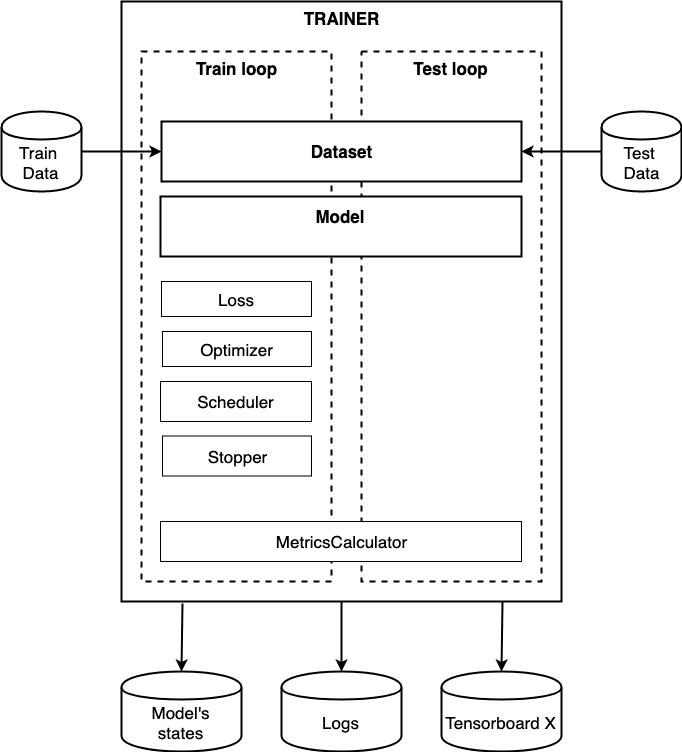
\includegraphics[width=0.95\linewidth]{Programm}
   	\end{center}
   	\caption{Структура программы для тренировки и обучения модели.}
   	\label{tikzpicture: programm}
\end{figure}


\subsection{Выбор метрики}

\indent
\indent
Прежде всего необходимо определиться, как количественно будет оцениваться
точность модели.Мы случайно выбрали 80\% данных 
для тренировки моделей, и 
20\% для их тестирования. В качестве метрик будем использовать 
классические для задачи классификации точность
 (\textit{accuracy}, не путать с \textit{precision}) и взвешенную точность:
выражения \ref{eq:accuracy} и \ref{eq:w_accuracy}.


\begin{equation}\label{eq:accuracy}
	   acc(\vec{y^{gt}}, \vec{y}) = \frac{1}{N}\sum_{i=1}^{N} \delta_{y_i^{gt}, y_i}
\end{equation}
где $\vec{y^{gt}}$ --- вектор номеров классов длинной $N$, 
$\vec{y}$ --- вектор предсказанных номеров классов длинной $N$,
$N$ --- количество рассматриваемых примеров,
$\delta$ --- символ Кронекера.

\begin{equation}\label{eq:w_accuracy}
	   acc_w(\vec{y^{gt}}, \vec{y}) = 
	   \frac{1}{C} \sum_{c}
	   \frac{1}{N_c}\sum_{\{i: y_i^{gt}\equiv c\}} \delta_{y_i^{gt}, y_i}
\end{equation}
где $N_c$ --- количество примеров из класса $c$, $C$ --- количество классов.
 

\indent
\indent
Таким образом, чтобы посчитать точность достаточно просто разделить
количество правильных ответов на общее количество ответов. Чтобы посчитать
взвешенную точность, необходимо вычислить точность для каждого класса
в отдельности, а затем усреднить полученные значения. В случае, если распределение
по классам в значительной степени неравномерное, отсутствие такого усреднения
приведет к тому, что значение метрики будет определяться точностью модели на
нескольких наиболее представленных классах. В данной работе мы будем
смотреть на значения обеих вариантов точности, но для принятия
решений о выборе модели приоритетной является взвешенная точность, так как в нашем наборе данных присутствует большой по размеру класс \textit{other}.


\section{Ход экспериментов}

\indent
\indent
Чтобы обучить модель оптимальным образом, сначала проведем серию
легковесных (с вычислительной точки зрения) экспериментов, чтобы определиться 
со значениями основных гиперпараметров. Затем попробуем улучшить целевую метрику
для лучшей модели, полученной на первом шаге.

\indent
\indent
Начнём с топологии нейронной сети. Будем выбирать из трех семейств архитектур:
 \textit{ResNet}, \textit{Inception} и \textit{VGG}; подробнее см. в разделе \ref{section:archs}.
Чтобы ускорить эксперименты уменьшим размер всех изображений до
$256 \times 256$ пикселей и не будем использовать аугментации во время тренировки.
Прекратим обучение после 50-ти
эпох\footnote{\textit{Эпохой} в машинном обучении называется один полный проход по
обучающему набору данных в процессе тренировки.}, либо остановимся досрочно,
если в течении 5-ти последних эпох от текущей не будет улучшено 
значение метрики хотя бы на 0.5\%. В качестве функции потерь используем
 перекрестную энтропию (см. раздел \ref{section: losses}),
 а в качестве оптимизатора параметров 
нейронной сети --- \textit{Adam} \cite{adam}, т.к. он не требует тонкой настройки
параметров. Кроме того, отследим время, которое 
понадобилось на обучение модели до остановки эксперимента 
по названному выше критерию.


\begin{table}[h]
    \begin{center}
        \begin{tabular}{c | c| c | c | c}
            \hline
            № & Архитектура & Точность & Взвешенная точность  & Время [мин] \\
            \hline
    
            1 & Inception v3 & 0.743 & 0.667 & 239 \\
            
            2 & VGG 11 & 0.678 & 0.565 & 154 \\
            
            3 & VGG 13 & 0.637 & 0.478 & 450 \\
            
            4 & ResNet 18 & 0.692 & 0.602 & 35 \\
            
            5 & ResNet 34 & 0.703 & 0.634 & 119 \\
            
            5 & ResNet 50 & 0.659 & 0.593 & 114 \\
    
            \hline
        \end{tabular}
    \end{center}
    \caption{Сравнение метрик для различных архитектур.}
    \label{tabular: arch_compare}
\end{table}


\indent
\indent
Как видно из результатов предварительных экспериментов
(таблица \ref{tabular: arch_compare}), наибольшую
точность показала архитектура \textit{Inception v3}. При этом 
\textit{ResNet34} уступает в точности незначительно, но требует
в 2 раза меньше времени на обучение, поэтому мы остановим свой
выбор на этой модели. 


Теперь попытаемся улучшить точность базовой модели,
используя различные техники тренировки и изменяя основные гиперпараметры.

\indent
\textbf{Оптимизатор}

\indent
Используем другой оптимизатор, например, \textit{SGD} с 
разными значениями скоростей обучения (\textit{learning rate}).
Кроме того, попробуем изменять скорость обучения в процессе тренировки:
будем её постепенно понижать и повышать.
Подразумевается, что такой подход может
помочь "вывести" функцию потерь из локального минимума. Данный
метод описан в статье 2017 года
\textit{Stochastic gradient descent with Warm Restarts}~\cite{cosine},
хотя его основная идея возникла ещё в 1983 году в публикации
\textit{Optimization by simulated annealing}~\cite{annealing}. В соответствии со
статьёй, скорость обучения изменяется по формуле \ref{eq:cosine}.

\begin{equation}\label{eq:cosine}
    lr_i = lr_{min} + \frac{1}{2} (lr_{max} - lr_{min}) (1 + \cos(\frac{i}{T} \pi ))
\end{equation}
где $lr$ -- скорость обучения,
$lr_{min}$ -- минимальная скорость обучения,
$lr_{max}$ -- максимальная скорость обучения,
$i$ -- номер текущей эпохи эпохи,
$T$ -- полупериод изменения скорости обучения. 

\indent
В настоящей работе использованы следующие параметры:
$lr_{min} = 0.001$, $lr_{max} = 0.1$ и $T = 3$, график изменения
скорости обучения изображен на рисунке \ref{tikzpicture: cosine}.

\begin{figure}[h!]
    \begin{center}
   	    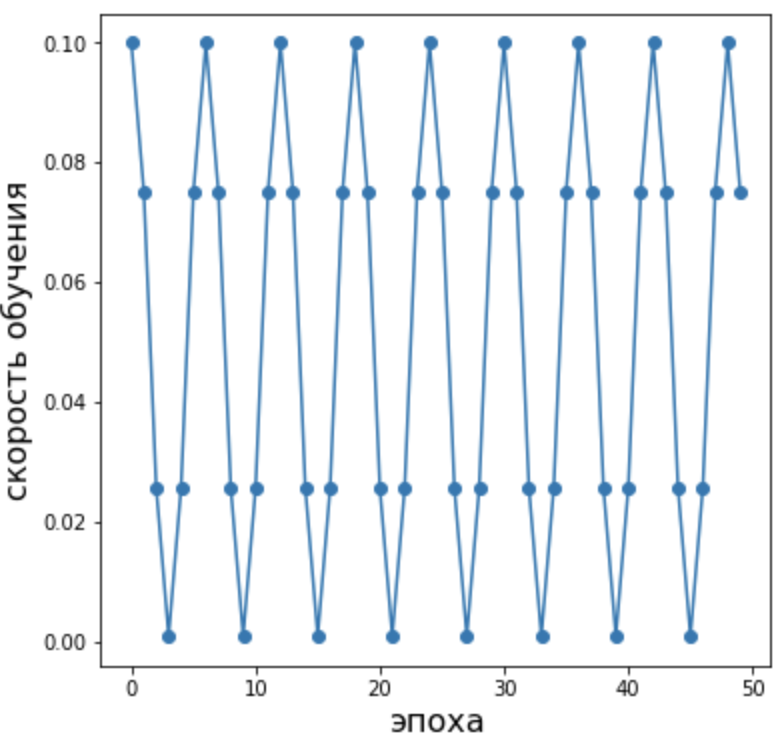
\includegraphics[width=0.5\linewidth]{cosine}
   	\end{center}
   	\caption{Изменение скорости обучения в процессе тренировки.}
   	\label{tikzpicture: cosine}
\end{figure}


\indent
\textbf{Размер изображений}

\indent
Попробуем уменьшать изображения не так сильно, 
до разрешения $512 \times 512$ вместо $256 \times 256 $.
С одной стороны, это сохранит больше информации, но с другой, увеличит 
количество пикселей в 4 раза, что уменьшит размер
%footnote
батча\footnote{\textit{Батчом} называется набор примеров, который передаётся
модели на обработку за один раз. При работе с изображениями размер батча 
ограничивается размером памяти видеокарты, на которой происходят вычисления.
Как правило, очередной шаг оптимизатора совершается после
прохождения батча, а не отдельного примера.}
%footnote
и замедлит тренировку.
Поэтому необходимо соблюсти баланс между приростом точности,
которого можно добиться использованием изображений большего размера,
и увеличением времени тренировки.

    
\indent
\textbf{Тренировочные аугментации}

\indent
Применим технику \textit{train time augmentations}, заключающуюся
в намеренном случайном искажении изображений, поступающих на вход модели 
в процессе обучения. Такие преобразования позволяют искусственно
"раздуть" размер тренировочного набора данных, увеличить его 
вариативность, что, в свою очередь, помогает бороться с переобучением
%footnote
модели\footnote{Переобучением называется ситуация, когда модель
запомнила правильные ответы для примеров из тренировочной выборки,
но не приобрела обобщающую способность. Другими словами, это ситуация,
когда модель имеет хорошее значение метрики на тренировочном наборе,
но очень плохое на тестовом.}.
%footnote
Но возникает вопрос о силе применяемых искажений.
Если трансформации слишком слабы, модель быстро адаптируются и её обобщающая 
способность не будет улучшена. Если слишком сильны, то визуальные паттерны, по
которым можно было бы классифицировать изображение, исчезнут.
Поступим следующим образом:
для каждого применяемого преобразования выберем некоторое базовое значение 
параметра, соответствующее преобразованию средней силы. 
Затем одновременно для всех преобразований будем изменять значения параметров,
кратно увеличивая или уменьшая выбранные базовые значения.
Будем говорить, что \textit{сила аугментаций = 1}, если используются трансформации 
с базовыми значениями параметров, \textit{сила аугментаций = 2} для удвоенного 
значения параметров и так далее. Перечислим используемые трансформации
и приведем базовые значения их параметров:

\begin{itemize}

    \item Поворот на угол от $-10$ до $+10$ градусов.

    \item Случайная обрезка краёв от $0$ до $10\%$ от размера изображения 
    (по вертикали и горизонтали).    
    
    \item Перенос на величину от $0$ до $10\%$ от размера изображения
    (по вертикали и горизонтали).
    
    \item Сдвиг на величину от $0$ до $10\%$ от размера изображения
    (по вертикали и горизонтали).
    
    \item Изменение отношения сторон на величину от $0$ до $15\%$
    (большей может стать как высота, так и ширина изображения).
    
    \item Случайное зеркальное отражение по горизонтали.
    
    \item Изменения яркости, контраста, оттенка и насыщенности.
    Степень задаётся числом от $0$ до $1$. Базовое значение $0.1$.
    
\end{itemize}
    
    
В качестве подходящих для данной задачи
искажений (трансформаций) используются:
горизонтальные зеркальные отражения (\textit{flips});
отбрасывание рамок случайного размера (\textit{crops});
цветовые и контрастные искажения;
разнообразные аффинные преобразования.
    
\indent
\textbf{Тестовые аугментации}

\indent
Применим технику \textit{test time augmentations}. 
Её смысл заключается в том, что на стадии использования модели
входное изображение
несколько раз копируется, и к копиям применяются различные 
искажения. После чего производится предсказание для каждой
копии, а в качестве окончательного ответа вычисляется, например, 
среднее значение по всем предсказаниям. Для многих задач таким образом
удается улучшить точность, но сложность вычислений линейно возрастает
с количеством созданных копий.

Результаты экспериментов, направленных на улучшение базовой модели
приведены в таблице \ref{tabular: train_tricks}. 15 эпох до остановки

\begin{table}[h]
    \begin{center}
        \begin{tabular}{c | c| c | c | c| c| c}
            \hline
            № & Оптимизатор & Сила & Разрешение & Точность & Взвешенная  & Время \\
            & & аугментаций & & & точность & [мин] \\
            \hline
    
           1 & Adam lr: 0.01 & 1 & $256 \times 256$ & 0.756 & 0.682 & 232 \\
           
           2 & SGD, lr: 0.01 & 1 & $256 \times 256 $ & 0.800 & 0.739 & 320 \\
           
           3 & SGD, lr: 0.1 & 1 & $256 \times 256 $ & 0.802 & 0.739 & 412 \\
           
           4 & SGD, lr: 0.01 & 3 & $256 \times 256 $ & 0.815 & 0.747 & 302 \\
           
           5 & SGD, lr: 0.01 & 1 & $512 \times 512 $ & 0.810 & 0.7811 & 1163 \\
               
           6 & SGD, lr: 0.01 & 5 & $256 \times 256$ & 0.771 & 0.695 & 369 \\
           
           7 & SGD, annealing & 1 & $256 \times 256$ & 0.8113 & 0.752 & 275 \\
            &  $T=3, lr_{max} = 0.1$ & & & & \\
           
            \hline
        \end{tabular}
    \end{center}
    \caption{Улучшение точности базовой модели (\textit{ResNet34}).}
    \label{tabular: train_tricks}
\end{table}



\subsection{Полученные результаты}

\indent
\indent
Чтобы лучше понять, как распределены ошибки обученной модели по классам,
построим матрицу ошибок: рисунок \ref{tikzpicture: conf_mat}.

\begin{figure}[h!]
    \begin{center}
   	    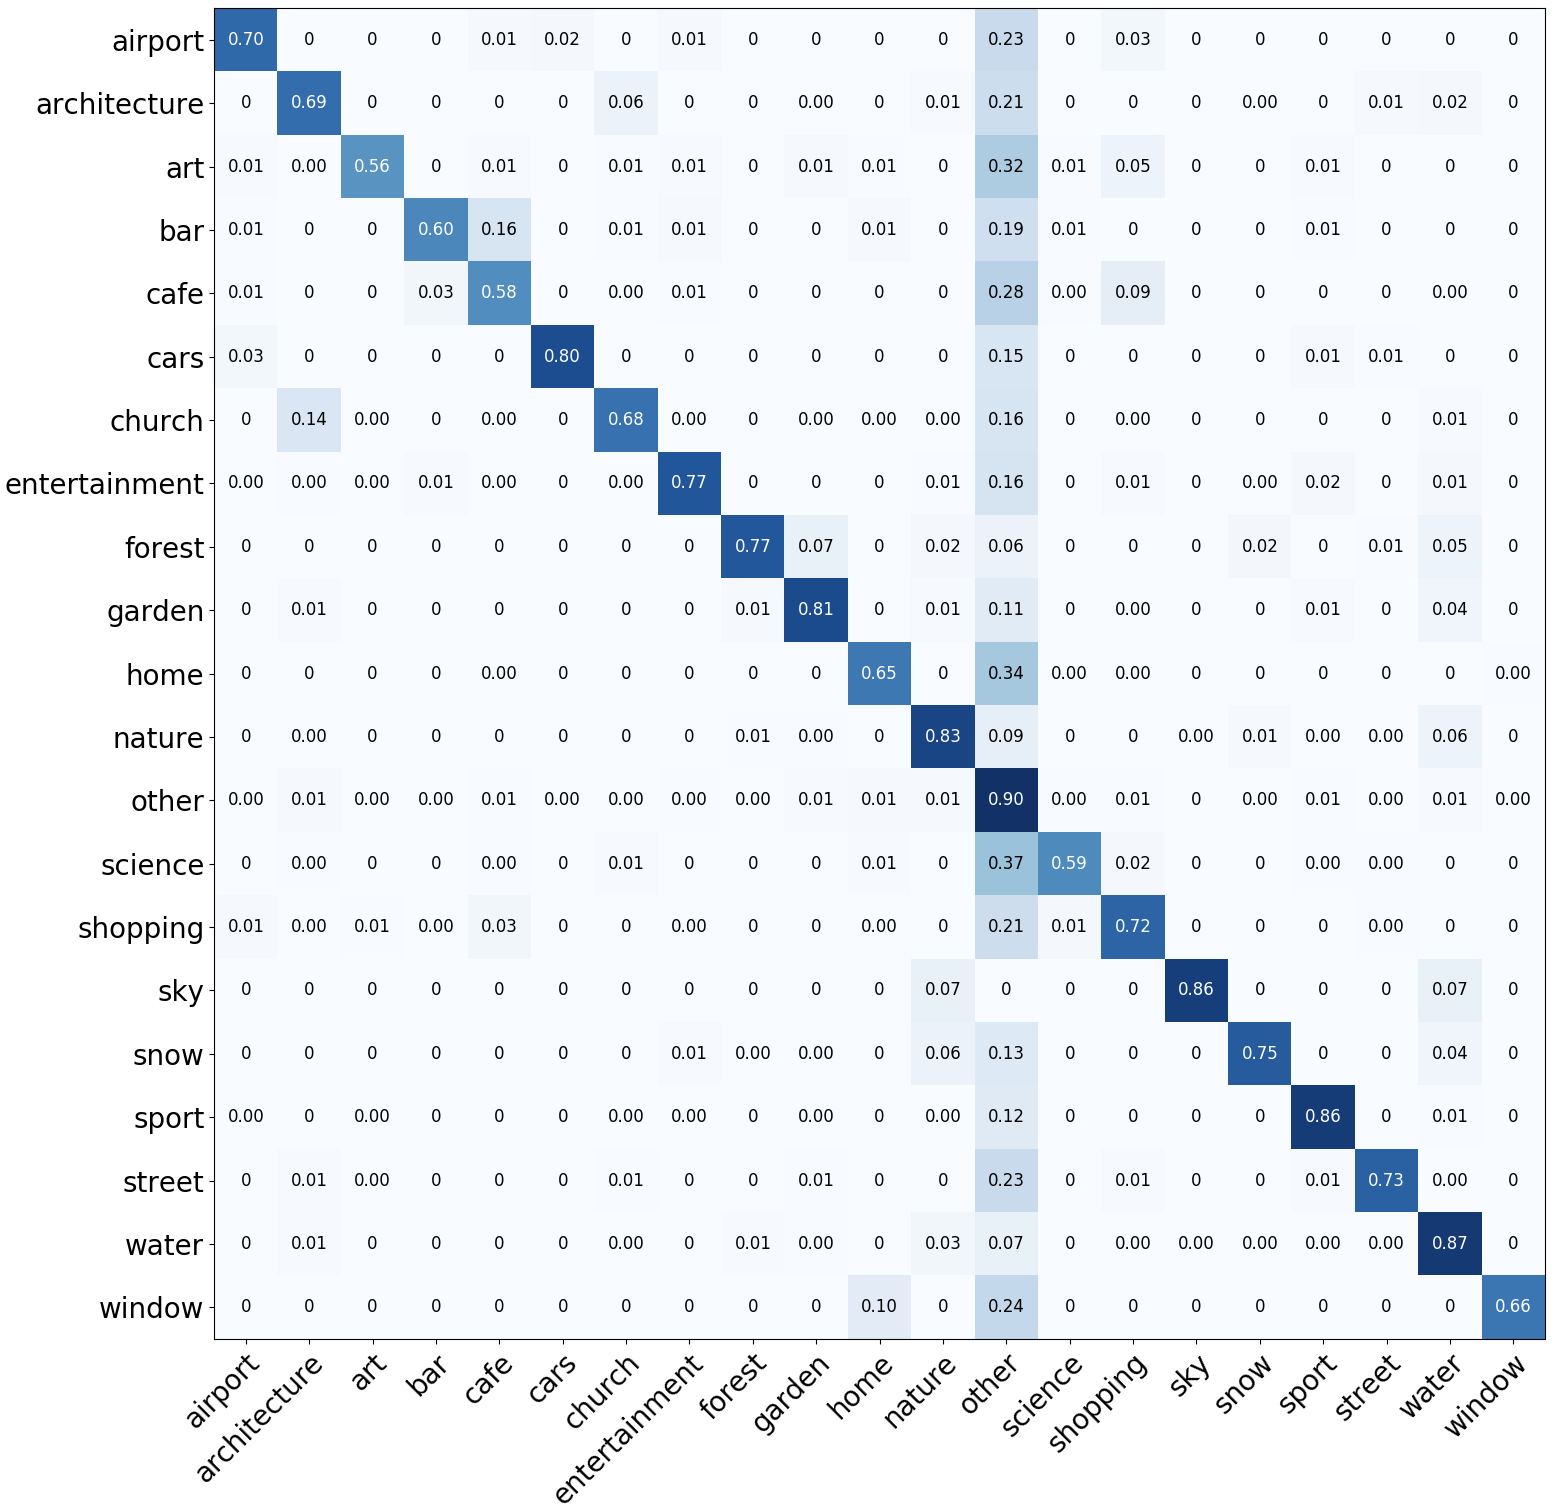
\includegraphics[width=0.95\linewidth]{conf_mat}
   	\end{center}
   	\caption{Матрица ошибок (\textit{confusion matrix}). Истинные метки 
   	               классов отложены по горизонтали, предсказанные -- по вертикали.}
   	\label{tikzpicture: conf_mat}
\end{figure}


\indent
\indent




\subsection{Обсуждение результатов}
todo
